\section{\textbf{思考問題}}
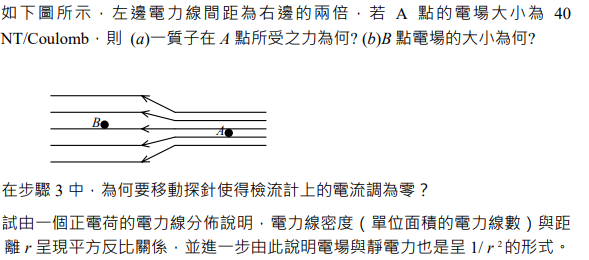
\includegraphics[width = 15cm ]{graph/image.png}
\begin{enumerate}
    \item 向左，40NT。
    \item 40NT/Coulomb。
    \item 表示該點電位與檢流計連接點電位相等。
    \item 因為點電荷的電力線在歐式幾何下為球形擴散，根據球表面積公式，電力線密度會與表面積成反比，與電場成正比，所以電場也就有$\frac{1}{r^2}$衰減的形式。
\end{enumerate}